\documentclass[a4paper]{article}

\usepackage{amsmath}
\usepackage{amssymb}
\usepackage{parskip}
\usepackage{fullpage}
\usepackage{hyperref}
\usepackage{bettelini}
\usepackage{stellar}
\usepackage{graphicx}
\usepackage{tikz}
\usepackage{fancybox}
\usepackage{makecell}
\usepackage[backend=bibtex]{biblatex}
\usepackage[version=4]{mhchem}

\hypersetup{
    colorlinks=true,
    linkcolor=black,
    urlcolor=blue,
    pdftitle={Chemistry},
    pdfpagemode=FullScreen,
}

\addbibresource{./references.bib}

\title{Chimica}
\author{Paolo Bettelini}
\date{}

\begin{document}

\maketitle
\tableofcontents

% 978.88.08.72527.1
% CHIMICA.BLU J.Brady

\pagebreak

\section{Chimica}

\sdefinition{Sistema}{
    Con \textit{sistema}
    si intende un oggetto o insieme di oggetti isolati
    di cui di studiano le prorpietà termodinamiche.
}

\sdefinition{Ambiente}{
    Con \textit{ambiente} si intende tutto ciò che si
    trova al di fuori del sistema e che è in grado
    di provocare in esso una modifica delle proprietà
    termodinamiche.
}

Sistema \(\subseteq\) Ambiente \(\subseteq\) Universo.

Un sistema può essere:
\begin{itemize}
    \item \textbf{aperto:} se scambia materia/energia con l'ambiente;
    \item \textbf{chiuso:} se scambia solo energia con l'ambiente;
    \item \textbf{osolato:} se non scambia nè energia nè material con l'ambiente.
\end{itemize}

Studiare un sistema significa descrivere le sue proprietà
\begin{itemize}
    \item \textbf{Qualitative:} possono essere definite senza avvalersi
    di misure.
    \item \textbf{Quantitative:} richiedono delle misure.
\end{itemize}
Le priorità misurabili sono delle \textit{grandezze}.

% TODO intensive / estensive

\subsection{Notazione scientifica}

La notazione scientifica viene espressa come
\[
    a \cdot 10^k,\quad a\in [1, 10)
\]

\pagebreak

\subsection{Sistema Internazionale}

\subsubsection{Grandezze fondamentali}

\begin{figure}[h]
    \centering
    \includegraphics[width=0.75\textwidth]{./si.png}
\end{figure}

\subsubsection{Grandezze derivate}

\begin{figure}[h]
    \centering
    \includegraphics[width=0.75\textwidth]{./grandezzederivate.png}
\end{figure}

\subsubsection{Misure}

\begin{figure}[h]
    \centering
    \includegraphics[width=0.75\textwidth]{./misure.png}
\end{figure}

\pagebreak

\section{Trasformazioni}

Le trasformazioni possono essere classificate come \textit{chimiche} o \textit{fisiche}.

\sdefinition{Trasformazione chimica}{
    Una \textit{trasformazione chimica}
    modifica la sostanza.
}

Nelle trasformazioni chimiche, gli atomi sono gli stessi ma gli elementi sono diversi.
Le particelle quindi mutano.

\sdefinition{Trasformazione fisica}{
    Una \textit{trasformazione fisica}
    non modifica la materia ma il suo stato.
}

Nelle trasformazioni fisiche, la materia mantiene le sue proprietà e rimane invariata.

\sexample{Trasformazioni chimiche}{
    \begin{itemize}
        \item Combustione di una candela (anche fisica).
        \item Cottura di un uovo (le proteine cambiano).
        \item Formazione della ruggina.
    \end{itemize}
}

\sexample{Trasformazioni fisica}{
    \begin{itemize}
        \item Combustione di una candela (anche chimica).
        \item Sbucciare una mela.
        \item Scaldare il tisolfato di sofio.
        \item Dissoluzione dello zucchero nell'acqua.
    \end{itemize}
}

\pagebreak

\section{Classificazione}

\subsection{Definizione}

\sdefinition{Sostanza pura elementare}{
    Una \textit{sostanza pura elementare} è composta da un solo tipo di elemento.
}

\sdefinition{Sostanza pura composta}{
    Una \textit{sostanza pura composta} è composta da un solo tipo di composto.
}

\sdefinition{Soluzione}{
    Una \textit{soluzione} è una sostanza composta da diversi tipi di composti
    in maniera omogenea.
}

\sexample{Sostanza pura composta}{
    Acqua (\(H_2O\))
}

\sexample{Sostanza pura elementare}{
    Azoto (\(N\))
}

\sexample{Soluzione}{
    \(50\% N + 50\% H_2\)
}

\begin{center}
    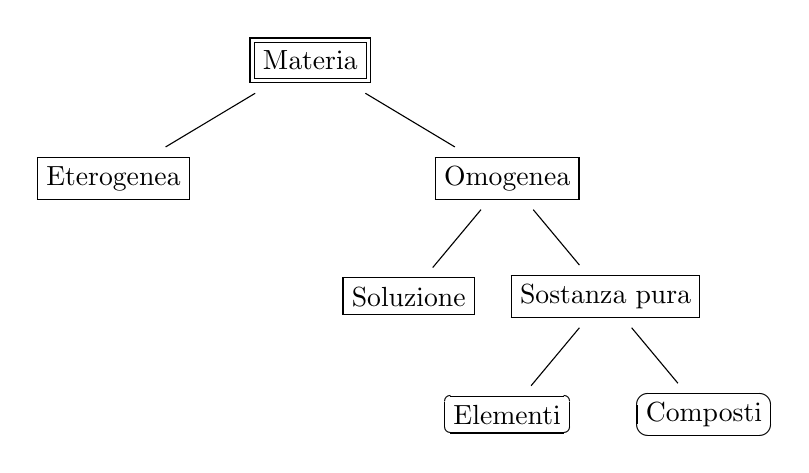
\begin{tikzpicture}[
        level 1/.style = {sibling distance = 5cm},
        level 2/.style = {sibling distance = 2.5cm}
    ]
    \node {\doublebox{Materia}}
        child {
            node {\fbox{Eterogenea}}
        }
        child {
            node {\fbox{Omogenea}}
            child {
                node {\fbox{Soluzione}}
            }
            child {
                node {\fbox{Sostanza pura}}
                child {
                    node {\ovalbox{Elementi}}
                }
                child {
                    node {\ovalbox{Composti}}
                }
            }
        };
    \end{tikzpicture}
\end{center}

\begin{itemize}
    \item La materia può essere classificata come materia \textit{eterogenea}
    e materia \textit{omogenea}.
    
    \item La materia omogenea può essere classificata come \textit{miscuglio omogeneo} (soluzione)
    oppure come \textit{sostanza pura}.
    
    \item Le sostanze pure possono essere classificati come \textit{elementi} oppure \textit{composti}.
\end{itemize}

\pagebreak

\subsection{Soluzioni (miscugli omogenei)}

Ogni soluzione è caratterizzata
da un \textit{soluto} ed un \textit{solvente}.

\sdefinition{Solubilità}{
    La \textit{solubilità} è la quantità massima che una sostanza
    può essere sciolta da una determinata quantità di solvente.
}
La solubilità dipende dalle proprietà chimica e altri fattori come la temperatura.
La solubilità dei gas diminuisce con l'aumento della temperatura.

Una soluzione è detta \textit{satura} o \textit{insatura}
se ha raggiunto il suo quantitativo massimo o meno.

Quando un soluto viene sciolto in un solvente, il volume della soluzione aumenta,
ma meno della somma dei due volumi. Questo è dato dal fatto che il soluto prende spazio fra le molecole del solvente.

\subsection{Tecniche di separazione}

\sdefinition{Decantazione}{
    La \textit{decantazione} si usa di solito per separare due liquidi di densità diversa
    sfruttando la gravità.
}

\sexample{Decantazione}{
    la separazione dell'olio e l'acqua.
}

\sdefinition{Distillazione}{
    La \textit{distillazione} sfrutta i diversi punti di ebollizione di due liquidi per separarli.
    La miscela viene riscaldata fino a quando solo uno delle due componenti diventa vapore, per poi
    spostarla e riaffreddarla.
}

\sdefinition{Cromatografia}{
    La \textit{cromatografia} sfrutta la tendenza delle sostanze a sciogliersi o interagire
    con diverse specie chimiche.
}

\sdefinition{Estrazione}{
    L'\textit{estrazione} si basa sulla maggiore o minore solubilità di un componente di un miscuglio in una certa miscela.
}

\sdefinition{Filtrazione}{
    TODO
}

\sdefinition{Centrifugazione}{
    TODO
}

\pagebreak

%\section{Reazioni chimica}
%Se una reazione chimica fra due elementi ha un rapporto di massa m, il rapporto delle massa atomiche è pari al rapporto, ma contando per il numero di atomi che reagiscono fra di loro.
% Se 1 atomo reasgisce con 1 atomo, il rapporto delle massa del reagente sarà il rapproto delle masse atomiche. 
% Legge delle proporzioni definite e costanti

%\pagebreak


\section{Radioactivity}

\subsection{Definition}

Radioactivity is a set of physical-nuclear processes
through which some unstable or radioactive atomic nuclei decay,
in a certain period of time called decay time.

An unstable nuclei will keep emitting radiations
and transmuting to other nuclei until the atom is stable.

\subsection{Decay}

The mass of a radioactive material will decrease exponentially.

\[
    M(t) = M_0 \cdot e^{-kt}
\]

\(M(t)\) is the mass (or number or particles)
after a certain time \(t\). \(M_0\) is the initial mass
and \(k\) is the rate of decay.

\subsection{Half-life}

The time of half-life is given by \(t_\frac{1}{2} = \frac{\ln 2}{k}\).

\begin{align*}
    \frac{1}{2}M_0 &= M_0 e^{-kt} \\
    \frac{1}{2} &= e^{-kt} \\
    \ln\left(\frac{1}{2}\right) &= -kt \\
    t &= \frac{\ln 2}{k}
\end{align*}

\subsection{Types of radiations}

There are three types of radiations that can be emitted by an unstable nucleai.

\paragraph{\(\alpha\) particles}

An \(\alpha\) particle is a helium nuclei. For example

\[
    \ce{^238_92U -> ^4_2\alpha{} + ^234_90Th}
\]

\paragraph{\(\beta\) particles}

There are two types of \(\beta{}\) particles. \(\beta{}^+\) and \(\beta{}^-\).
A \(\beta{}^+\) particle is emitted when the nuclei is unstable due to
having too many protons, whist the \(\beta{}^-\) one is emitted when it has
too many neutrons.

\[
    \begin{cases}
        \beta{}^+,\quad \ce{^0_{+1}e} \text{ (positron)} \\
        \beta{}^-,\quad \ce{^0_{-1}e} \text{ (electron)}
    \end{cases}
\]

\paragraph{\(\gamma\) particles}

\(\gamma\) rays are photons of electromagnetic energy. They have \(0\) mass and \(0\) charge.

\pagebreak

\section{Energy levels}

An electron is a fundamental particle. It is attracted by protons in the
atom nuclei but they repelled by one another.
The places where the electrons are found around the nuclei are called
\textit{atomic orbitals.} \\
There are two types of orbitals, \textbf{s} and \textbf{p}.
Electrons in \textbf{s} orbitals can be measured to be in a spherical region around the nuclei,
whilst electrons in \textbf{p} orbitals have a dumbell-shaped position region
(zero-probability of being measured at the center of the nuclei).
An orbital can host up to two electrons.
Orbitals are grouped in different zones.
Eletrons in zones closer to the center have lower energy and the amount of energy
to move an electron from its zone to the next one is constant.

At the lower energy there is a single \(1\text{s}\) orbital that can hold two electrons.
At the next energy level, there are four orbitals:
\(2\text{s}\), \(2\text{p}1\), \(2\text{p}2\) and \(2\text{s}3\) for up to 8 electrons at this level of energy.
In larger atoms electrons can be found at the level \(3\text{s}\) and \(3\text{p}\)

Atoms where the level with most energy is not completly empty or completly full is unstable.
The excess electorns are called valence electrons. An atom may share, give or take electrons
with other atoms to become stable.

\subsection{Ionic bond}

An ionic bond is a transfer of valence electrons between metallic atoms and non-metallic atoms.
The outcome of this process is a positive ion (more protons than electrons)
and a negative ion (more electrons than protons). These ions attract each other often
forming a crystal structure.

\subsection{Metallic bond}

A metallic bond is a transfer of valence electrons between metallic atoms.
The valence electrons continually move from one atom to another and are not
associated with any specific pair of atoms. This creates a structure of positive ions
which conducts electricity (since electrons can freely move).

\subsection{Covalent bond}

A covalent bond is a sharing of pairs of electrons between non-metallic atoms.
A covalent bond happens just between two atoms, it can be simple, double or triple (2, 4, 6 total shared electrons).

\subsection{Electronegativity}

Electronegativity is a measure of an atom's ability to attract shared electrons to itself.
The type of bond if given by the different of electronegativity between two atoms.
\begin{itemize}
    \item \(0\) - \(0.4\): Pure covalent bond
    \item \(0.4\) - \(1.7\): Polar covalent bond
    \item \(1.7\) -: Ionic bond
\end{itemize}

\pagebreak

\section{Acids}

The pH level is a measure of the acidity or alkalinity of a solution. It is a logarithmic scale that ranges from 0 to 14, with 7 being considered neutral. A pH value below 7 indicates acidity, while a pH value above 7 indicates alkalinity.

The pH scale is based on the concentration of hydrogen ions (\(\text{H}^+\)) in a solution. An acidic solution has a higher concentration of \(\text{H}^+\) ions, while an alkaline solution has a lower concentration of \(\text{H}^+\) ions. The pH scale is logarithmic..

OH stands for hydroxide ion, which is a negatively charged molecule consisting of one oxygen atom and one hydrogen atom. It is the conjugate base of water (\(\text{H}_2\text{O}\)) and plays a role in determining the pH level of a solution. The concentration of \(\text{OH}^-\) ions in a solution is directly related to its alkalinity, as the higher the concentration of \(\text{OH}^-\) ions, the more alkaline the solution is.

\begin{align*}
    \text{pH} &= - \log_{10}(\text{H}^+) \\
    \text{pOH} &= - \log_{10}(\text{OH}^-) \\
    \text{pH} + \text{pOH} &= 14 \\
\end{align*}

\pagebreak

\section{Redox}

\subsection{Definizione}

\sdefinition{Reazione di ossidoriduzione} {
    Le reazioni di \textit{ossidoriduzione} (\textit{redox}) sono una reazione chimica in cui gli elettroni
    vengono trasferiti tra due reagenti che vi partecipano.
    Le reazioni di ossidoriduzione sono composte da un
    \begin{itemize}
        \item \textit{agente riducente:} la sostanza che si ossida donando elettroni;
        \item \textit{agente ossidante:} la sostanza ossida prendendo elettroni.
    \end{itemize}
}

Una reazione redox comporta un cambiamento nello stato di ossidazione di uno o più atomi.

\subsection{Numeri di ossidazione}

\sdefinition{Numero di ossidazione}{
    Il \textit{numero di ossidazione} è la carica elettrica virtuale che si può
    attribuire a un atomo o a uno ione impegnato in un legame chimico,
    immaginando di spostare tutti gli elettroni del legame sull'atomo più elettronegativo.
}

Lo stato di ossidazione o numero di ossidazione di un atomo in una molecola rappresenta la sua capacità di perdere o guadagnare
elettroni in una reazione chimica. In una molecola neutra, la somma degli stati di ossidazione di tutti gli atomi è
sempre uguale a zero. Ciò significa che la somma degli elettroni persi da alcuni atomi è uguale alla somma
degli elettroni acquistati da altri atomi. In una molecola ha l'atomo con la più alta elettronegatività
sempre il numero di ossidazione negativo.

\begin{enumerate}
    \item Elementi singoli e liberi hanno sempre un numero di ossidazione di \(0\);
    \item ioni monoatomici hanno sempre un numero di ossidazione pari alla propria carica;
    \item il fluoro ha sempre numero di ossidazione di \(-1\) essendo il più elettronegativo;
    \item la somma di tutti i numeri di ossidazione degli atomi in una molecola deve essere
        uguale alla carica della particella;
    \item l'idrogeno ha numero di ossidazione \(+1\) nei composti con i non metalli e \(-1\)
        nei composti con i metalli;
    \item l'ossigeno ha quasi sempre un numero di ossidazione di \(-2\), \(-1\) per i perossidi;
    \item i metalli dei gruppi I e II hannno rispetivamente numeri di ossidazione di \(+1\) e \(+2\);
    \item gli alogeni hanno numero di ossidazione \(-1\) nei composti con i metalli e un numero di ossidazione
        positivo quando si legano a \(O\) o \(F\).
\end{enumerate}

%i metalli dei primi gruppi tendono a cedere i propri elettroni esterni OSSIDANDOSI;
%i non metalli, molto elettronegativi, acquistano invece elettroni, RIDUCENDOSI;

Se lo stato di ossidazione aumenta, la molecola si ossida (perde elettroni). \\
Se lo stato di ossidazione diminuisce, la molecola si riduce (acquista elettroni).


\subsection{Reazione spontanea}

\sdefinition{Reazione spontanea}{
    Una reazione è \textit{spontanea} se procede spontaneamentes.
}

\subsection{Esercizi}

\sexercise{Trova il numero di ossidazione}{
    \begin{align*}
        &\,\bullet \text{NaCLO}_3 & +1, +5, -2 &&&&&&\\
        &\,\bullet \text{SnCL}_4 & +4, -1 &&&&&&\\
        &\,\bullet \text{MnO}_4^{2-} & +6, -2 &&&&&&\\
        &\,\bullet \text{MnO}_2 & +4, -2 &&&&&&\\
        &\,\bullet \text{H}_2\text{O}_2 & 1, -1&&&&&&
    \end{align*}
    L'idrogeno ha solo un elettrone, per cui il numero di ossidazione dell'ossigeno deve essere
    ridotto.
}

\sexercise{la combustione del metano è una reazione di ossidoriduzione?}{
    La reazione
    \[ \text{CH}_4 + \text{O}_2 \rightarrow \text{CH}_2 + \text{H}_2\text{O} \]
    ha numeri di ossidazione
    \begin{align*}
        &\,\bullet \text{CH}_4 & -4,+1 &&&&&&\\
        &\,\bullet \text{O}_2 & 0 &&&&&&\\
        &\,\bullet \text{CH}_2 & -2,+1 &&&&&&\\
        &\,\bullet \text{H}_2\text{O} & +1,-2&&&&&&
    \end{align*}
}

% DImostrare che la combustione  del metano  (CH_4) è una redox.

% O2 -> O has number 0
% H2O2 -> O has number -1

\pagebreak

\section{Polarità}

\sdefinition{Polarità}{
    Una molecola è polare (non pura) se vi è una carica parziale.
}
Il legale ionico è quello più polare perché strappa un elettrone. \\
La differenza di elettronegatività deve essere da 0 a 0.45 per essere puro
(il valore 0.45 è scelto per considerare il legame CH come apolare).

Quando una molecola è fatta solo da 2 atomi, 
se il legame è polare, la molecola è polare.
Quando ci sono più legami, è necessario almeno un legame polare
ma la molecola non deve essere simmetrica, altrimenti le cariche parziali si annullano.

Le sostanze apolari si sciolgono in solventi apolari, e quelli polari in quelli polari.
Di conseguenza, oer essere solubile in acqua una moecola deve essere polare.


\section{Lgami secondari (forze intermolecolari)}

\sdefinition{Forza forte}{
    Legame covalente, metallico o ionico.
}
\sdefinition{Forza debole}{
    Forze di Van der Walls, forze di Londom, ponte a idrogeno.
}

I legami secondari (deboli, intermolecolari) sono responsabili delle interazioni fra molecole uguali o diverse tra loro,
o anche fra parti diverse della stessa molecola.

Se il legame non è un ponte idrogeno ma è lo stesso principio, di dice dipolo-dipolo.
Infatti, il legame ponte idrogeno è dipolo-dipolo ma ha un nome speicfico.
Le forze di Van der Walls sono i legami dipolo-dipolo.
Quando le interazioni non sono polari si parla di forze di London.

\subsection{Dissoluzione del sale nell'acqua}

L'acqua ed il sale Na\(^{+}\)Cl\(^{-}\) inducono un polo.
Le cariche positive dell'acqua (idrogeno) vengono attratte da quelle negative
del cloruro, mentre quelle negative dell'acqua (ossigeno)
vengono attratti da quelle negative del sale (Na).
Il cristallo del sale viene quindi separato dalle forze
esercitate dai dipoli dell'acqua.

Il motivo per cui il cristallo si spacca e non le molecole di acqua
è dato dal fatto che l'energia delle interazioni deboli è più che sufficiente
per compensare l'energia necessaria per rompere le interazioni ione-ione
nel cristallo e alcuni legami idrogeno acqua-acqua.

\subsection{Forze deboli nell'H2O}

I ponti a idrogeno creano una struttura esagonale con le molecole d'acqua,
formando il ghiaccio.
Questo è il motivo per cui la struttura dei giocchi di neve è esagonale.
Quando l'acqua è gassosa non ci sono queste forze debole, e quando sono
liquide ce ne sono poche e casuali.
Il motivo è che l'energia aumuenta con l'aumentare della temperatura,
e per cui con temperature troppe alte, questa energia spacca i legami deboli.

Il sale nell'acqua salata rende più difficile la creazione di ponti a idrogeno.

% anche il motivo per cui l'acqua ghiaccia solo sopra
% foto esagono e fiocchi di neve

\pagebreak

\subsection{Sviluppo del calore nelle reazioni}

La rottura di un legame necessita di energia, mentre
la formazione di legami libera energia.

\begin{center}
\begin{figure}[h]
    \centering
    \includegraphics[width=\textwidth]{./cov_bond_energy.png}
\end{figure}
\end{center}

\sdefinition{Entalpia}{
    L'\textit{entalpia} è la quantità di energia interna che un sistema
    termodinamico può scambiare con l'ambiente.
}

\sdefinition{Reazione esotermica}{
    Una \textit{reazione esotermica} è una reazione che libera energia termica.   
}

La reazione esotermica possiede le seguenti caratteristiche:
\begin{itemize}
    \item la reazione rilascia calore;
    \item l'ambiente circostance si scalda;
    \item l'entalpia \(\Delta H_{\text{reazione}} < 0\);
    \item i legami che si formano nei prodotti sono più forti di quelli che si rompono nei reagenti;
    \item i prodotti hanno energia inferiore rispetto ai reagenti.
\end{itemize}

\sdefinition{Reazione endotermica}{
    Una \textit{reazione endotermica} è una reazione che assorbe energia termica.   
}

La reazione esotermica possiede le seguenti caratteristiche:
\begin{itemize}
    \item l'entalpia \(\Delta H_{\text{reazione}} > 0\);
\end{itemize}

In una reazione esotermica all'equilibrio chimico,
aumentando la temperatura si sposta tale equilibrio verso i reagenti,
per cui la reazione inversa è favorita rispetto alla reazione diretta
per temperature elevate. Il segno della variazione di entalpia
(che è un aspetto termodinamico) indica semplicemente la predisposizione della
reazione chimica ad evolversi in senso diretto o inverso,
mentre per conoscere la velocità di reazione è necessario considerare gli aspetti cinetici.

L'energia è direttamente proporzionale alle mole, e quindi alla massa.

Il calore acquisito o rilasciato da un corpo è durettamente proporzionale
alla variazione di temperatura a cui va incontro e si ricava dall'espressione
\[
    Q = mc\Delta T
\]
dove \(c\) è il calore specifico.

\sdefinition{Entalpia standard di formazione}{
    L'\textit{entalpia standard di formazione}
    di una sostanza, o \textit{calore standard di formazione}
    è la quantità di calore assorbita o liberata quando una mole della sostanza
    viene formata, a \(25 {}^\circ \) C e 1 atm, dai suoi elementi nei loro stati standard.
}

Conoscendo l'entalpia delle sostanze, per qualunque
reazione possiamo calcolare direttamente la variazione di energia di reazione.
\[
    \Delta H^\circ_{\text{reazione}} =
    \sum_{f \in \text{prodotti}} \left( \Delta H^\circ_f \right) -
    \sum_{f \in \text{reagenti}} \left( \Delta H^\circ_f \right) 
\]

L'Entalpia Standard di Formazione,
\(\Delta H^\circ_f\), di una sostanza è il \(\Delta H^\circ\)
della sua reazione di formazione.

Una sostanza pura ha sempre entalpia di formazione \(\Delta H^\circ_f = 0\).

\pagebreak

\section{Thermodinamica chimica}

\sdefinition{Energia di attivazione}{
    L'\textit{energia di attivazione} è l'energia necessaria
    a far accadere una reazione chimica.
}

\sdefinition{Catalizzatore}{
    Un \textit{catalizzatore} è
    una sostanza in grado di influenzare la
    velocità di una reazione chimica senza essere consumata.
}

Il catalizzatore accelera la reazione abbassando l'energia
di attivazione dando la possibilità che si realizzi un nuovo
percorso che porta ai prodotti, caratterizzato da uno stadio
cineticamente determinante con una minor energia di
attivazione rispetto a quello della reazione non catalizzata.

\sdefinition{Velocità di reazione}{
    Per rappresentare la \textit{velocità di reazione}, descriviamo la
    variazione nel tempo della concentrazione di una specie
    presente nell'equazione chimica
    \[
        v
        = - \frac{1}{a} \frac{d[A]}{dt}
        = - \frac{1}{b} \frac{d[B]}{dt}
        = \frac{1}{p} \frac{d[P]}{dt}
        = \frac{1}{q} \frac{d[Q]}{dt}
    \]
    dove \(a,b,p,q\) sono i coefficienti stechiometrici
    per i reagenti \(A\) e \(B\) e i prodotti \(P\) e \(Q\).
}

\subsection{Teoria degli urti efficaci}

\sdefinition{Teoria degli urti}{
    La \textit{teoria degli urti}
    indica che 
    la velocità di una reazione è
    proporzionale al numero di urti efficaci che avvengono
    nell'unità di tempo fra le molecole dei reagenti.
    Un urto è \textit{efficace} solo se porta alla formazione delle
    molecole dei prodotti.
}

\begin{center}
\begin{figure}[th]
    \centering
    \includegraphics[width=\textwidth]{./urti.png}
\end{figure}
\end{center}

Affinché gli urti siano efficaci occorre che le particelle che
entrano in contatto abbiano un'energia cinetica molecolare
minima, ossia l'energia di attivazione.

Dopo un urto, le molecole rallentano: la loro energia
cinetica diminuisce e si trasforma in energia potenziale.

\pagebreak

\sdefinition{Stato di transizione}{
    Con \textit{stato di transizione} si intende
    il momento della reazione in cui il
    legame tra i reagenti è parzialmente rotto e il nuovo
    legame è parzialmente formato (complesso attivato).
}

La sua energia corrisponde al punto più alto del diagramma dell'energia potenziale.

\begin{center}
\begin{figure}[th]
    \centering
    \includegraphics[width=\textwidth]{./reaction.png}
\end{figure}
\end{center}

\pagebreak

\subsection{Equilibrio}

In una reazione chimica, vi sono sia reazioni dirette che inverse.
Questo siginfica che è si giungere ad un equilibrio dove
il numero di reagenti e quello di prodotti tendono ad essere in equilibrio,
con scambi continui fra i due.

\begin{center}
\begin{figure}[th]
    \centering
    \includegraphics[width=\textwidth]{./equilibrio}
\end{figure}
\end{center}

Il grafico della reazione può essere quindi diviso in \textit{regione cinetica}
e \textit{regione di equilibrio}. 
Nell'equilibrio \textit{dinamico} le molecole continuano costantemente a
cambiare, e la velocità di reazione diretta diventa quella di reazione indiretta.
Nell'\textit{equilibrio statico} le reazioni si fermano.

% TODO: 2 reagenti e un prodotto. Possiamo cmq avere una regione di equilibrio
% Osserviamo che l'andamento di crescita e di diminuzione
% non è più speculare. Se ce ne sono solo 2 è speculare.

% Spostare una reazione verso destra, significa che il reagente si trasforma in prodotto.
% C'è più prodotto che reagente al momento dell'equilibrio.
% diagramma Alcuni diagrammi (RP) con le 3 immagini

\sdefinition{Legge di azione di massa}{
    Data una reazione generica
    \[
        dD + eE \rightleftharpoons fF + gG
    \]
    l'\textit{espressione dell'azione di massa} è
    \[ \frac{{[F]}^g{[G]}^g}{{[D]}^d{[E]}^e} = K \]
    dove \(K\)  è la \textit{costante di equilibrio} e relaziona
    le concentrazioni delle singole specie chimiche all'equilibrio.
}

Le dimensioni di \(K\) variano con la stechiometria della reazione.\\
Ogni reazione possiede una costante di equilibrio caratteristica,
il cui valore dipende solo dalla temperatura.

Se \(K\) è grande, la reazione è spostata a destra,
e vi sono pochi reagenti e tanti prodotti.
Di conseguenza, se il \(K\) è grandisimo la reazione inversa è quasi
ininfluente, perché ve n'è pochissima.

\sexample{
    La creazione di ammoniaca \(NH_3\) possiede come reagenti \(N_2\) e \(H_2\).
    La reazione termochimica è data da
    \[
        N_{2(\text{g})} + H_{2(\text{g})}   \rightleftharpoons NH_{3(\text{g})}      
    \]
    Siccome abbiamo \(\Delta H = -46.2 \frac{\text{kJ}}{\text{mol}}\),
    possiamo convenientemente bilanciare l'equazione in maniera tale da avere 1 mole di ammoniaca
    \[
        \frac{1}{2}N_{2(\text{g})} + \frac{3}{2}H_{2(\text{g})}   \rightleftharpoons NH_{3(\text{g})}
    \]
    Partendo da un punto della reazione di equilibrio,
    aggiungere \(H_2\) o \(N_2\) porterà uno sbilanciamento dell'equilibrio.
    Di conseguenza,
    I valori di \(N_2\) e \(H_2\) diminuiranno, favorendo la creazione di ammoniaca.
    Allo stesso modo, togliere dell'ammoniaca porta alla creazione di nuova ammoniaca, a scapito
    di \(H_2\) e \(N_2\).
    Togliendo uno dei reagenti, la concentrazione di ammoniaca scende per riequilibrare la reazione,
    e quella dell'altro reagente sale, e viceversa.
    I rapporti fra le differenze di concentrazioni che bilanciano la reazione dopo
    uno squilibrio sono proporzionali ai coefficienti stechiometrici:
    togliendo dell'ammoniaca, la concentrazione di \(H_2\) diminuirà maggiormente di quella di \(N_2\).
}

I modi per aumentare la concentrazione di un prodotto sono:
\begin{enumerate}
    \item Aumentare i reagenti;
    \item Aumentare il volume del reattore;
    \item Aumentare la temperatura (se \(\Delta H > 0\)).
        Aumentando la temperatura,
        i prodotti aumentano se la reazione è endotermica (\(\Delta H > 0\)),
        mentre i prodotti diminuiscono se è esotermica (\(\Delta H < 0\));
    \item Aumentare la pressione (se ho più molti nei reagenti che nei prodotti).
        Se si aumenta la pressione, la miscela all'equilibrio
        cambia composizione e diminuisce il numero totale di molecole allo stato gassoso presenti nel recipiente.
        Non c'è effetto della pressione
        se non c'è variazione nel numero di molecole durante la reazione.
        L'aumento della pressione sposta l'equilirio verso la parte della reazione che possiede meno molti di gas.
        Questo è dato dal fatto che il sistema deve bilanciare l'aumento della pressione, spostando
        la reazione verso dove vi sono meno moli di gas (nei reagenti o nei prodotti);
    \item Togliere prodotto (per spostare l'equilibrio e fare generare altro prodotto, anche se meno di quanto ne ho tolto,
        ma il quantitativo totale aumenta).
\end{enumerate}

Il catalizzatore non aumenta la concentrazione di un prodotto, bensì solo la concentrazione.
La temperatura è l'unico fattore al quale cambia la costante \(K\).

\pagebreak

\subsection{Principio di Le Chatelier}

\sdefinition{Principio di Le Chatelier}{
    Secondo \textit{principio di Le Chatelier},
    ogni sistema tende a reagire ad una perturbazione impostagli
    dall'esterno minimizzandone gli effetti.
}

\sexercise{Spiega l'effetto ottenuto sull'equilibrio da una reazione}{
    \[ O_{2(\text{g})} + N_{2(\text{g})} \rightleftharpoons 2NO_{2(\text{g})} \]
    \begin{itemize}
        \item \textbf{aumento della temperatura:}
            se la reazione diretta è endotermica, scaldare favorirà la produzione di prodotti,
            mentre se la reazione è esotermica, raffreddare favorirà la formazione di prodotti;
        \item \textbf{diminuzione della pressione:}
            ci sono due moli di gas sia a destra che a sinistra, per cui non abbiamo nessun influsso.
        \item \textbf{aumento della concentrazione di ossigeno:}
            viene favorita la produzione di prodotti (spostamento verso destra);
        \item \textbf{diminuzione pressione parziale di N\({}_2\):}
            viene diminuita la concentrazione di azoto, e per cui avremo meno prodotti;
        \item \textbf{aumento della concentrazione NO:}
            aumentano i reagenti (viene favorita la reazione inversa);
        \item \textbf{presenza di un catalizzatore:}
            l'equilibrio non cambia.
    \end{itemize}
}

\pagebreak

\section{Isotopi dell'idrogeno}

\subsection{Deuterio}

Il primo isotopo dell'idrogeno è il \textit{deuterio}, indicato con \(D\) o \(^2H\).
A differenza dell'idrogeno comune, il deuterio possiede un neutrone nel nucleo oltre al protone.
A causa di questa caratteristica, il deuterio ha una massa atomica leggermente superiore rispetto all'idrogeno normale.
Il deuterio è utilizzato in varie applicazioni, come nei reattori nucleari per la produzione di energia e come tracciatore in studi scientifici e biologici. 

\subsection{Trizio}

Il secondo isotopo dell'idrogeno è è il trizio, indicato con \(T\) o \(^3H\).
A differenza dell'idrogeno comune, il deuterio possiede due neutroni nel nucleo oltre al protone.
A causa di questa composizione nucleare, il trizio ha una massa atomica maggiore rispetto agli altri isotopi dell'idrogeno.
Il trizio è radioattivo e decade nel tempo con una emivita di circa 12,3 anni, emettendo particelle beta.

\section{Acqua con deuterio e trizio}

È possibile ottenere dell'acqua, \(H_2O\), utilizzando gli isotopi \(D\) e \(T\) al posto di \(H\).

Queste sostanze sono chiamate \textit{acqua pesante} (\(D_2O\)) e
\textit{acqua superpesante} (\(T_2O\)).

\subsection{Densità}

\begin{center}
    \bgroup{}
    \def\arraystretch{1.25}
    \begin{tabular}{ |c|c|c|c| }
        \hline
        & \textbf{Acqua} & \textbf{Acqua pesante} & \textbf{Acqua Superpesante} \\
        \hline
        \textbf{Liquido (g/cm\(^3\))} & 0.997 & 1.11 & 1.20 \\
        \hline
        \textbf{Solido (g/cm\(^3\))} & 0.9168 & 1.105 & ? \\
        \hline
    \end{tabular}
    \egroup{}
\end{center}

Normalmente, le molecole dell'acqua che ghiaccia si organizzano, e creano molti spazi (caso unico).
Questo implica che il ghiaccio abbia una densità minore dell'acqua, per cui esso galleggia se immerso nell'acqua.

Possiamo quindi notare dalla tabella come la versione solida dell'acqua pesante galleggi
nell'acqua normale \cite{deuterated-water}.

\nocite{*} % cite all entries

\printbibliography

% reagenti -> prodotti + E (eso)
% reagenti + E -> prodott (endo)

\end{document}

APPUNTI ESPE:
Fare frasi complete con la maiuscola
Nell'esercizio scrivere i passaggi con le unità di misura in maniera sequenziale.
I risultati metteteli in una frase: es. si sono prodotti 5g di merda